\documentclass[12pt]{article}

\usepackage{sbc-template}

\usepackage{graphicx,url}
\usepackage{listings}
\usepackage{subfigure}

\RequirePackage[vlined,titlenumbered,algo2e,ruled]{algorithm2e} 

\usepackage[T1]{fontenc}
     
\sloppy

\title{Debugging Techniques for Distributed R-Trees}

\author{S�vio Teles\inst{1}, Jose Ferreira de S. Filho\inst{1}}

\address{Instituto de Inform�tica -- Universidade Federal de Goi�s (UFG) \\
  Alameda Palmeiras, Quadra D, C�mpus Samambaia \\
  131 - CEP 74001-970 -- Goi�nia -- GO -- Brazil
\email{savioteles@gmail.com, jkairos@gmail.com}
}

\begin{document} 

\maketitle

\begin{abstract}
 The growing availability of data and the number of users have motivated the emergence of distributed algorithms to process spatial operations efficiently. 
 Those distributed algorithms are based on distributed indexes for efficient processing. 
 Researches and ongoing work use R-Trees as distributed spatial index structure for indexing and retrieval of objects. 
 However, distributed indexes based on R-Trees have a challenge: How debugging a distributed index based on an R-Tree? 
 In the last years many researches have been published on distributed algorithms and distributed processing. 
 However, none of them has addressed the debugging of a distributed R-Tree index. 
 This paper presents a new algorithm for debugging a distributed R-Tree index, hereinafter RDebug. 
 This algorithm has been used on DistGeo, a spatial platform, and to visualize the algorithms' output a graphic tool was created.
\end{abstract}

\section{Introduction}
\label{sec:intro}

The Internet has revolutionized the computer and Geographical Information Systems (GIS) like nothing before. In fact the Internet brought big changes how systems store, retrieve and analyze spatial data. The ever-increasing of the large geospatial datasets and the widely application of the complex geocomputation make the parallel processing of GIS an important component of high-performance computing. Thus, spatial distributed applications came on the scene. We define a spatial distributed application as one which software components located at networked computers communicate and coordinate their actions for geoprocessing.

In order to handle spatial data efficiently, a database system needs an index mechanism that will help it retrieve data items quickly according to their spatial locations. An R-tree is a dynamic index structure, which meets this need and is broadly used by in GIS. Generally, the R-Tree index is built and processed in a single machine. However, process an R-Tree in a single machine is not feasible because of the huge size of the geospatial datasets. Thus, many researches such as  \cite{an1999storing,dedsi,zhong2012towards}, show that a distributed index structure spanning the workstations can provide an efficient shared storage structure that can be used to gather geographic information more efficiently.

A big challenge though has arisen of spanning the R-Tree index structure among computers: How debug a distributed R-Tree index structure? 

Debugging is an essential step in the development process, albeit often neglected in the development of distributed applications due to the fact that distributed systems complicate the already difficult task of debugging.

In recent years, researchers have been developed some helpful debugging techniques for distributed environment. Nevertheless, we have not found any technique to debug a distributed R-Tree. In this paper, we propose a debugging technique to debug the data insertion in an R-Tree, besides of debugging the quality of the index built on the cluster.

The debug method, hereafter called RDebug, uses the distributed index structure to aggregate debugging information. RDebug is used by DistGeo, a shared-nothing platform for distributed spatial algorithms processing. We also created a graphical tool to visualize the debugging information and the R-Tree index structure. 

The main achievements of this paper are:

\begin{itemize}
  \item RDebug - A debugging technique to the data insertion algorithm in a distributed R-Tree.
  \item DistGeo - A Shared-nothing platform, without point of failure, to process distributed spatial algorithms of an R-Tree.
  \item A graphical tool to visualize debugging information and the distributed R-Tree index.
\end{itemize}

The rest of the paper is structured as follows. Section \ref{sec:spatial_dist} describes the distributed processing of spatial algorithms, Section \ref{sec:rdebug} presents our approach for distributed R-Tree debugging. In Section \ref{sec:related}, we briefly give an overview of the use of debugging techniques for distributed environments and the view of the distributed spatial algorithms. Finally, we close the paper with some concluding remarks in Section \ref{sec:conclusion}.

\section{Distributed Processing of Spatial Algorithms}

\subsection{Data Structures for Spatial Data Processing}

	Over the last decades spatial data indexing techniques have been the subject of many researches, which originated diverse data structures, such as: KD-Tree [Bentley 1975], Hilbert R-Tree [Kamel and Faloutsos 1994] and R-Tree [Guttman 1984].
	
	R-Trees were proposed by Antonin Guttman in 1984 and have found significant use in both theoretical and applied contexts, they are tree data structures used for spatial access methods, i.e, for multi-dimensional information such as geographical coordinates, rectangles, polygons. Similar to the B-Tree [Comer 1979], the R-Tree is also a balanced search tree (so all leaf nodes are at the same height).

	The key idea of the data structure is to group nearby objects and represent them with their minimum bounding rectangle (MBR) in the next higher level of the tree; the "R" in R-tree is for rectangle. Since all objects lie within this bounding rectangle, a query that does not intersect the bounding rectangle also cannot intersect any of the contained objects. At the leaf level, each rectangle describes a single object; at higher levels the aggregation of an increasing number of objects. This can also be seen as an increasingly coarse approximation of the data set.
	
	R*-Trees are a variant of R-Trees used for indexing spatial information. R*-trees have slightly higher construction cost than standard R-trees, as the data may need to be reinserted; but the resulting tree will usually have a better query performance. Like the standard R-tree, it can store both point and spatial data. It was proposed by Norbert Beckmann, Hans-Peter Kriegel, Ralf Schneider, and Bernhard Seeger in 1990. R*-Trees are the data structure described in this paper.
Figure 1 illustrates the hierarchical structure of an R-Tree with a root node, internal nodes (N1...2 C N3...6) and leaves (N3...6 C a...i). The Upper Top of Figure 1 shows MBRs grouping spatial objects of a..a i in sets by their co-location. The bottom of Figure 1 illustrates the R-Tree representation. Each node stores at most M and at least m <=M/2 entries [Guttman 1984].

\begin{figure}[ht]
\centering
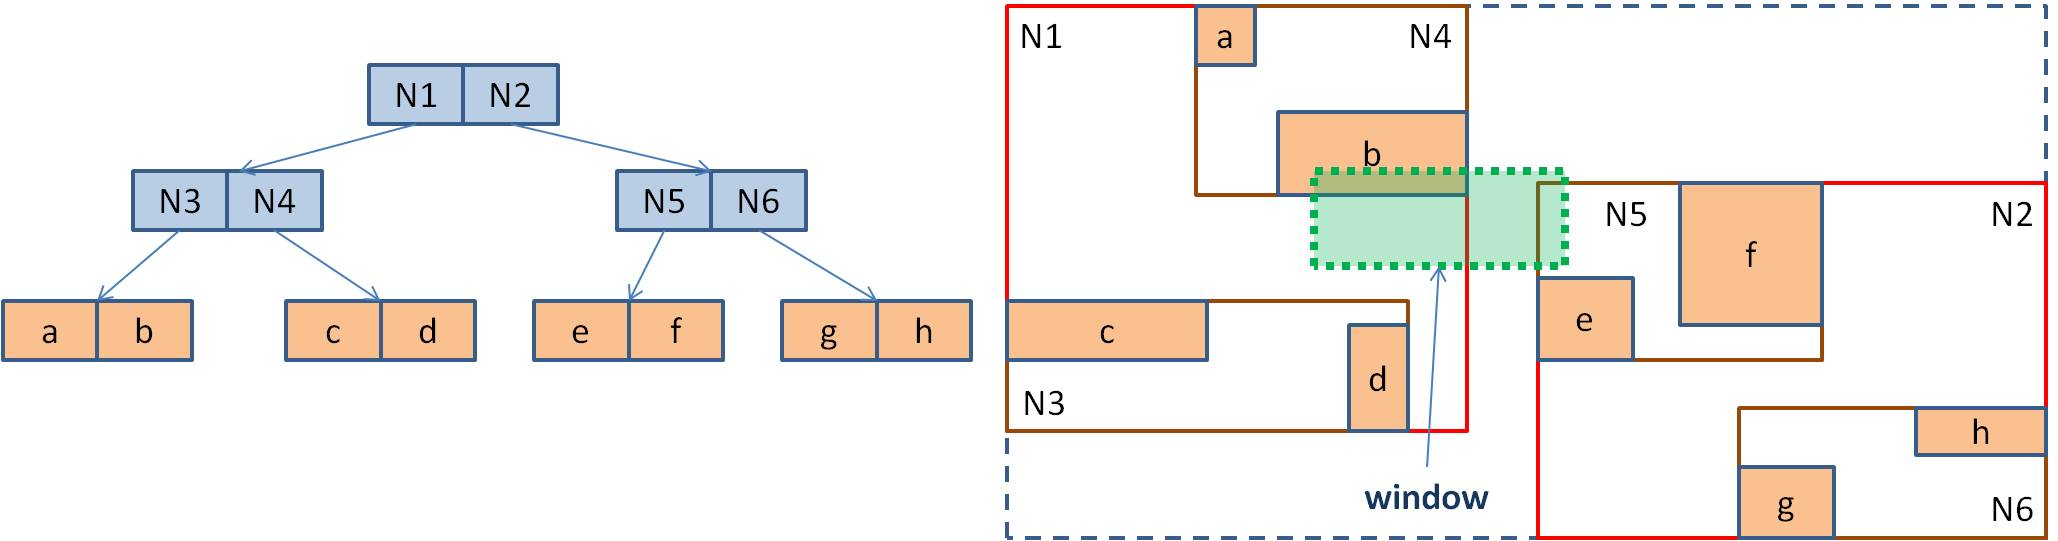
\includegraphics[width=.5\textwidth]{r-tree-structure.png}
\caption{R-Tree Structure}
\label{fig:R-Tree Structure}
\end{figure}

The input is a search rectangle (Query box). Searching is quite similar to searching in a B+ tree. The search starts from the root node of the tree. Every internal node contains a set of rectangles and pointers to the corresponding child node and every leaf node contains the rectangles of spatial objects (the pointer to some spatial object can be there). For every rectangle in a node, it has to be decided if it overlaps the search rectangle or not. If yes, the corresponding child node has to be searched also. Searching is done in a recursively until all overlapping nodes have been traversed. When a leaf node is reached, the contained bounding boxes (rectangles) are tested against the search rectangle and their objects (if there are any) are put into the result set if they lie within the search rectangle.
	
	Dead space is a space which is indexed but does not contain data. In Figure 1, N1 area is an example of dead space. Dead spaces cause the search go into false sub-trees. In figure 1, window K represents the intersection between the MBR dead space and N2, the search walks through the sub-tree of N2, although this sub-tree does not contain any data to return.
Overlapping areas are regions of intersection between polygons. The area between N3 and N4 in Figure 1 is an example of overlapping. Less overlapping reduces the amount of sub-trees accessed during r-tree traversal. The overlapping area between N3 and N4 in Figure 1, forces the traversal of the two sub-trees, degrading the performance of R-Tree [Guttman 1984, Beckmann et al. 1990].

\subsection{DistGeo: A Platform of Distributed Spatial Operations for Geoprocessing}

There are two important requirements for processing data in shared-nothing (cluster) [DeWitt and Gray 1992] architectures, First divide the data in partitions. The second requirement is distribute this partitions in the cluster nodes. For spatial datasets, we use the same idea of partitions, and the partitions distribution considers the geographic co-location among the polygons to speed up the searching algorithm.

Figure 2 illustrates the structure of a Distributed R-Tree in a cluster. The partitioning it is performed grouping the nodes in cluster and creating the indexes according to the R-Tree structure. The lines in figure 2 show the need for message exchange to reach the sub-trees during the algorithm processing.

\begin{figure}[ht]
\centering
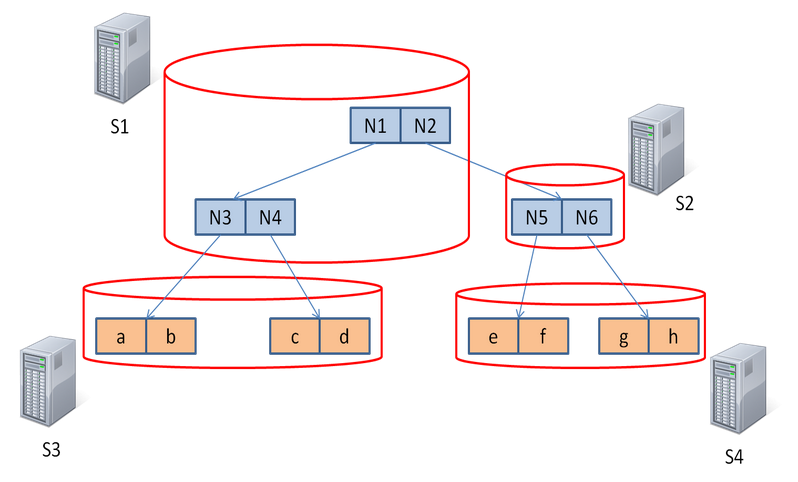
\includegraphics[width=.5\textwidth]{r-tree-partiotioning.png}
\caption{R-Tree Partitioning in a shared-nothing architecture}
\label{fig: R-Tree Partitioning in a shared-nothing architecture}
\end{figure}

Insertions and searching in a distributed R-Tree are similar to the non-distributed version, except for:
i) The need of message exchange to access the distributed partitions
ii) Concurrency control and consistency due to the parallel processing in the cluster.
	The data distribution among the distributed partitions in the cluster is both the main factor to the parallel processing and also the main challenge when building the distributed index.
	Quality of index is another factor, which influences the communication. An index with high quality reduces the searching space and the sub-tress access leading to less number of message exchange.
	This section describes the main architecture decisions and some implementation details that molds the challenges when constructing a solution for distributed Geo-processing.
	The distributed index has been built according to the taxonomy defined in [An et al. 1999], as follows:
	i) Allocation Unit: block - A partition is created for every R-Tree node;
	ii) Allocation Frequency: overflow - In the insert process, new partitions are created when a node in the tree needs to split;
	iii) Distribution Policy: balanced - To keep the tree balanced the partitions are distributed among the cluster nodes.
	DistGeo is based on the shared-nothing architecture, which the nodes do not share CPU, hard disk and memory and the communication relies on message exchange. Figure 3 depicts DistGeo plataform based on peer-to-peer model, with the data manage by the cluster presented as a ring topology. It is divided in ranges of keys, which are managed for each node of the cluster. To a node join the ring it must first receive a range
	The range of keys are known by each node in the cluster. For instance, in a ring representation, whose key set start with 0 till 100, if we have 4 nodes in the cluster, the division would be done as shown below:
\begin{enumerate}
 \item node 1: 0-25
  \item node 2: 25-50
  \item node 3: 50-75
  \item node 4: 75-100
\end{enumerate}

If we want to search for one object with key 34, we certainly should look on the node 2.

\begin{figure}[ht]
\centering
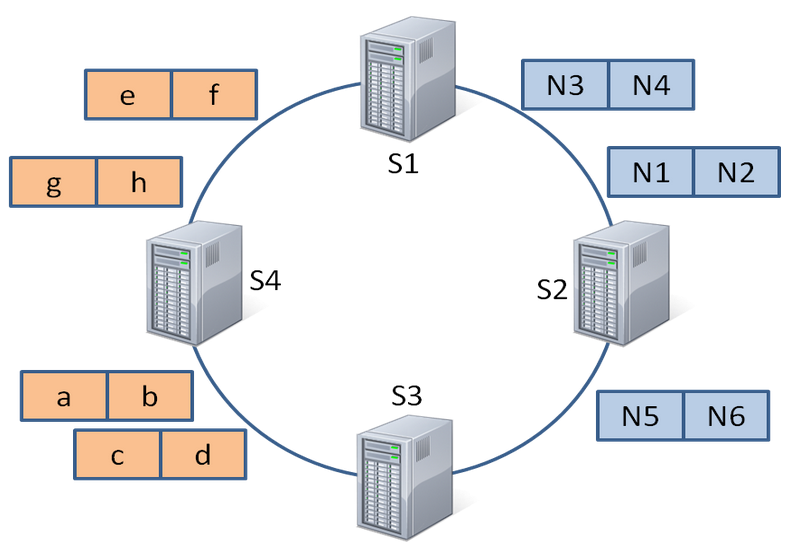
\includegraphics[width=.5\textwidth]{figure3.png}
\caption{Figure 3}
\label{fig: Figure 3}
\end{figure}

	Reliability and fault-tolerance are implemented storing the R-Tree nodes in multiple nodes in the cluster. Each node N receives a key, which is used to store the node in a server S responsible for ring range, replicating the node N to the next two servers in S (clockwise).
	
	Data replication is equally important. If a message is sent to a bode N, in the moment of R-Tree traversal an active server is elected, and replicates the data in this node to further requisition processing.
	
	The Gossip protocol, which every cluster node exchanges information among themselves is used by DistGeo for service discovery and knowing the status of the cluster's nodes. Gossip protocol. Every second a message is exchanged among three nodes in the cluster, consequently every cluster's node have knowledge of each other.
	
	Read/Write operations may be performed in any node of the cluster. When a request is made to a cluster's node, it becomes the coordinator of the operation requested by the client. The coordinator works as a proxy between the client and the cluster's nodes. In a distributed R-Tree, the requests are always sent to cluster's node, which stores the root node of the R-tree.

\section{A Technique for Debugging A Distributed R-Tree}
\label{sec:rdebug}

	Spatial index debugging is a big challenge in a distributed R-Tree and this section describes a new technique RDebug, which allows debugging the index building of an R-Tree.
	
	The R-tree index building follows a top-down approach, in other words, the index is always built from root to leaves. Debugging the index reliability as the index is built is a non-trivial task, and the aim of this paper is to show a technique for index debugging after it has been created. Common challenges when working with an R-Tree are: i) Reliability of the nodes replicas of the R-Tree, ii) ensure that the MBR of the parent nodes intersect the MBR of their children, iii) the existence of duplicated nodes or being referenced by more than one parent node, and iv) if the value M and m of the nodes are compliant with the R-Tree descriptions as shown in Section \ref{sec:spatial_dist}. Furthermore, it is possible to access index data to help in its optimization as dead space and overlapping area.

	Algorithm \ref{alg:rdebug} shows the RDebug technique for debugging the distributed spatial index, using the index structure itself. The algorithm has two steps:
1) The algorithm processing is similar to the search in an R-Tree; 2) The algorithm does the inverse of a search in an R-Tree appending information to the distributed index.

	The first step, called S1 [Search sub-trees] (lines 1 - 11), the Algorithm \ref{alg:rdebug} traverses every node of the R-Tree starting from the root node to the leaves. Its purpose is to spread the debugging algorithm. The first request is sent to any server, which stores a replica of the root node.

	If the node $T$ is not a leaf (lines 2 - 8), then the number of children entries is stored to control the number of expected answers to this node in the second step of the algorithm. This information is stored in a shared memory accessed by all servers with a replica of $T$. Lines 4 -7, show that for every entry $E$ in the node, a message is sent (continuing step S1) to any server that holds a replica of the child node of $E$, carrying on the first step in the children nodes. If the node is a leaf, the second step, named S2 [Aggregation] is started.

	Second step aim (lines 12 - 41) is to aggregate the information used for future debugging. This step receives the debugging information of every child node of $T$. Therefore, for a given node $T$ with $n$ children, the second step is invoked $n$ times in the node $T$.

	The index itself is used to aggregate this information, the computational resources of the cluster helps improve the debugging information aggregation time. The index reverse structure allows, besides of spanning the aggregation information processing, build the debugging aggregation information, as one node of the R-Tree is responsible to aggregate only the information of its children. 

	Line 13 verifies the consistency of $T$ in the servers that store any replica of $T$. Line 14 verifies the consistency of $M$ and $m$. Lines 16 and 17 calculate the dead space and overlapping area for each node of the R-tree. Those information help the insertion algorithm designer analyze the quality of the built index. Beside this, lines 18 - 22, we have information of the MBRs of each node for every entry of the node. This information can be used as an input to a tool capable of visualizing the index of the R-Tree.
	
	If the aggregation step is being executed in the leaves, then if  $T$ is the root node (lines 24 - 26), the node information are sent to the client application. IF $T$ is not the root node, in line 27, the information are sent to the parent node of $T$. If the aggregation step is in an internal node (lines 29 - 43), the algorithm aggregates the information of the children nodes. Line 29, the algorithm receives the information sent by the child node. Line 30, verifies if the MBR of the entry that points to the child node is indeed the same MBR sent by the child node.
	
	The information of the children nodes are stored in a shared memory, with concurrency control, by the replicas of $T$. Hence, line 31, those information are accessed from the shared memory. Line 32, adds the data processed from lines 29 and 30. Line 33, acquires the number of children nodes that sent debugging information in the shared memory of replicas $T$. This information is stored in the variable $count$ and $count$ is decremented to let the other replicas know.
	
	If every node has sent the answer, the variable count then will hold the value 0 and lines 35-39 are processed. If $T$ is the root node, then the information are sent to the client application, otherwise, those information are sent to the parent node of $T$. If the variable $count$ is greater than 0, then the client information are stored in the shared memory.	
		
\medskip
\begin{center}
\begin{minipage}{1\textwidth}
\begin{algorithm2e}[H]
\SetAlFnt{\small\sf}
 \DontPrintSemicolon
 \LinesNumbered
\SetAlgoLined
 \BlankLine
 \Entrada{$T$ reference to root node of R-Tree $tree$}
 \Saida{Debugging information about distributed R-Tree $tree$}
 \BlankLine
	
 S1 [Search subtrees]

\eIf{$T$ is not leaf}{
  store the number of child entries in each replica server of T\;
	
	\For{each entry $E$ in $T$} {
		$server \leftarrow $ choose one server, randomically,  that store one replica of $E$\;
		send msg to $server$ to process the node child of $E$ on step S1\;
	}
}
{
  verifiy the consistency of $T$ in others replicas\;
	Invoke step S2 [Aggregation]\;
}

S2 [Aggregation]

$replica\_consistency \Leftarrow$ verifiy the consistency of $T$ in others replicas\;
$node\_consistency \Leftarrow$	verify the consistency of $M$ and $m$ values of  $T$\;
add in $informations$: $replica\_consistency$ and $node\_consistency$\;

$overlap \Leftarrow$ overlap area of $T$\;
$dead\_area \Leftarrow$ dead area of $T$\;
$bound \Leftarrow$ MBR of $T$\;
$list \Leftarrow \emptyset$\;

\For{for each entry $E$ in $T$}{
	add the $MBR$ of $E$ in $list$\;
}

\eIf{$T$ is leaf}{
 \If{$T$ is root}{
		send response with R-Tree nodes information to app client\;
	}
	{
		send msg with $informations$ to parent of $T$\;
	}
}
{
	  $entry\_info \Leftarrow$ information sent by child node\;
    $mbr\_consistent \Leftarrow$ verify if the bound of the child node is equal to bound of entry of T that points to this child\;
		$informations \Leftarrow$ the child information stored on shared memory by replicas of $T$\;
    add in $informations$: $entries\_info$, and $mbr\_consistent$\;
		
		$count \Leftarrow$ retrieve the number of entries child which not sent a debugging response and decrement by 1 unit\;
		
    \eIf{$count$ == 0}{
        \eIf{$T$ is root}{
           send response with $informations$ to app client\;
        }
				{
				   send msg with $informations$ to parent of $T$\;
				}    
		}
		{
			store $informations$ on shared memory\;
		}
            
}
\caption{$RDebug(T)$ 
\label {alg:rdebug}}
\end{algorithm2e}
\end{minipage}
\end{center}

The algorithm \ref{alg:rdebug} was implemented in the DistGeo platform to collect the debugging information of the built distributed R-tree. Those information are used in the platform to find out indexing issues and to optimize the R-tree index for searching. Figure 4.1, shows a graphical tool created to visualize the structure of the distributed R-Tree index, using as the input the information generated by the distributed debugging algorithm in DistGeo platform.

[Colocar a Figura aqui!!]

With the aid of RDebug \ref{alg:rdebug} algorithm, it is possible debug the searching algorithms of an R-Tree. E.g: The Window Query algorithm shown on Section \ref{sub:spatialdata}. To tweak RDebug to Window Query, it is only needed add an window query in the first step and gather the aggregation information of the accessed nodes. Whereas, the algorithms that access diverse R-Trees, such as Spatial Join, need a deep change, as the algorithms can go through different paths.

\section{Related work}
\label{sec:related}

Researches on distributed spatial data either show techniques to debug distributed applications in general or techniques for R-tree distributed processing, 
but none adressed both issues.
The Section \ref{dist_debug} shows the distributed debugging researches and \ref{spatialdist} describes researches of platforms for processing distributed spatial algorithms.
	
\subsection{Distributed Debugging Techniques}
\label{dist_debug}

In \cite{remeD2011} the author breaks down debuggers in two main families: log-based debuggers (also known as post-mortem debuggers) and breakpoint-based debuggers 
(also known as online debuggers). 
Log-based debuggers insert log statements in the code to be able to generate a trace log during its execution. 
Breakpoint-based debuggers, on the other hand, execute the program in the debug mode that allows programs to pause/resume the execution at certain points, 
inspect the state and the perform step-by-step execution. 

Several breakpoint-based debuggers have been designed for parallel programs using message passing communication including p2d2 \cite{p2d21996}, TotalView \cite{totalView2009}, and Amoeba \cite{amoeba1989}. 
These debuggers offer the traditional commands to stop, inspect and execute step-by-step a running program. 
Some of them allow to set breakpoints on statements of one process (e.g. \cite{totalView2009}) or a set of processes (e.g. \cite{p2d21996}, \cite{amoeba1989}). 

A great body of concurrent and parallel debugging techniques are event-based. 
Event-based debuggers \cite{mcdowell1989Debugging} conceive the execution of a program as a sequence of events. 
The debugger records the history of the events generated by the application, which can then be used to either browse the events once the application is finished \cite{xtrace2007,causeway2009}, 
or to replay the execution to recreate the conditions under which the bug was observed. 
 
\cite{cheung1990Framework} describes a process for distributed debugging in general and does not focus on a specific debugger or a particular technique, 
the paper focus is on defining a step-by-step approach to tackle distributed debugging independent of the environment. 
	
\subsection{Distributed Spatial Algorithms}
\label{spatialdist}

This Section describes briefly the researches which present the use of parallelism in order to improve the response time of the spatial algorithms. 
M-RTree \cite{koudas1996declustering} was the first published paper, 
which shows a shared-nothing architecture, with a master and several workstations connected to a LAN network. 
The master machine can be a bottleneck because it handles and client requests and moreover merges the answers of the slaves and send to client machines. 
A similar technique was found on MC-RTree \cite{schnitzer1999master} and \cite{an1999storing}, which show the same problems on master machine.

Hadoop-GIS \cite{kerr2009alternative} shows a scalable and high performance spatial data warehousing system for running large scale spatial queries on Hadoop. 
However, it does not use index to process the spatial operations. \cite{dedsi} presents a platform to process distributed spatial operations. 
Although, the solution proposed in \cite{dedsi} implements a distributed index, it is not scalable, since every message go through the replicated master node. 
\cite{de2013processamento} shows a hybrid peer-to-peer platform, which comprehends a set of machines for naming resolution that could be
a bottleneck in the system.   

\cite{xie2008two} introduces a two-phase load-balancing scheme for the parallel GIS operations in distributed environment.
\cite{zhang2009spatial} describes MapReduce and shows how spatial queries can be naturally expressed in this model.
However, it is only indicated for non-indexed datasets. 

A number of techniques and platforms have been proposed for handling spatial big data.
Nevertheless, none of the researches propose a technique for distributed spatial index debugging of an R-Tree.
Besides, none of them propose a platform using a peer-to-peer approach for processing distributed spatial algorithms as found on DistGeo platform (Section \ref{sub:dist_geo}).

\section{Conclusion}
\label{sec:conclusion}

DistGeo platform presents an approach for processing the distributed spatial operations through the distributed R-Tree index. Due to the distributed processing nature on this platform an issue arises: Debugging the insertion algorithm when the R-tree nodes a distributed in a cluster.

We have seen researches on spatial data processing and distributed debugging, but none of them propose techniques for debugging the spatial algorithms of an R-Tree. In this paper, we present RDebug, a technique for debugging the distributed index building of an R-Tree. RDebug, uses the R-Tree index itself to gather the debug information. The information gathering is done in the R-Tree index using a down-top traversal in the tree. Utilizing the distributed index itself, the data gathering can be achieve in a distributed way, improving the debugging algorithm efficiency.

RDebug, has been implemented in DistGeo platform. The R-Tree nodes are distributed and replicated over the cluster. Thus, RDebug can be processed without bottlenecks and point of failures. Besides, the R-Tree replicated nodes in the cluster allow load-balancing in the distributed R-Tree index traversal. During the traversal, at every node access of the R-Tree, the traversal might go to a node of the cluster with less workload increasing RDebug performance. The information exchange of the machines statuses is done trough the Gossip algorithm.

A graphical tool has been created to visualize the structure of the distributed R-Tree index and the debugging information about the index building. With these input we can identify discrepancies in the index building and optimize it.

Ongoing work includes modify the RDebug algorithm to debug the Window Query and Join Query searching algorithms. The RDebug algorithm is easily adapted to gather debugging information for Window Query. Whereas, for Join Query algorithm, RDebug must be changed considerably, since the traversal is processed in two different distributed R-Trees. Another ongoing work is to realize performance tests of the RDebug algorithm in DistGeo platform.

\bibliographystyle{sbc}
\bibliography{sbc-template}

\end{document}